\documentclass[11pt]{article}
\usepackage{amsmath, amsfonts, amssymb}
\usepackage[margin=1in]{geometry}
\usepackage{graphicx}

\begin{document}

\title{ELCT562 PA \#1}
\author{Jacob Vaught}
\date{\today}
\maketitle

\section*{Problem 1}
To calculate the TX power in dBW and dBm, we use the formulas:
\begin{align*}
    \text{dBW} &= 10 \cdot \log_{10}(P_{\text{tx}}) \\
    \text{dBm} &= 10 \cdot \log_{10}(P_{\text{tx}} \times 1000)
\end{align*}
Given \( P_{\text{tx}} = 0.1 \) W, the calculations are as follows:
\begin{align*}
    \text{dBW} &= 10 \cdot \log_{10}(0.1) = -10 \text{ dBW} \\
    \text{dBm} &= 10 \cdot \log_{10}(0.1 \times 1000) = 20 \text{ dBm}
\end{align*}

\section*{Problem 2}
For the coverage range, we use two models: Free-Space Path Loss (FSPL) Model and Simplified Path Loss Model.

\subsection*{Free-Space Path Loss (FSPL) Model}
The Free-Space Path Loss (FSPL) model is used to predict the attenuation of a radio signal as it travels through free space. The FSPL is given by the formula:
\[
L = 20 \log_{10}(d) + 20 \log_{10}(f) + 20 \log_{10}\left(\frac{4\pi}{c}\right) - G_{t} - G_{r}
\]
where \(L\) is the path loss in dB, \(d\) is the distance in meters, \(f\) is the frequency in Hz, \(c\) is the speed of light in m/s, \(G_{t}\) is the transmit antenna gain in dBi, and \(G_{r}\) is the receive antenna gain in dBi.
\newline

Given the desired received power is \(-70\) dBm, the frequency \(f = 2.45 \cdot 10^9\) Hz (2.45 GHz), transmit antenna gain \(G_{t} = 9\) dBi, and receive antenna gain \(G_{r} = 2\) dBi, we can rearrange the formula to find the maximum distance \(d\) at which the received power would be \(-70\) dBm. The calculation is as follows:
\[
P_{tx}-P_{rx} = 90 \text{ dBm} = 20 \log_{10}(d) + 20 \log_{10}(2.45 \cdot 10^9 \text{ Hz}) + 20 \log_{10}\left(\frac{4\pi}{3\cdot 10^8}\right) - 9 \text{ dBi} - 2 \text{ dBi}
\]
Simplifying the equation, we isolate \( \log_{10}(d) \):
\[
20 \log_{10}(d) = 90 \text{ dBm} - 20 \log_{10}(2.45 \cdot 10^9 \text{ Hz}) - 20 \log_{10}\left(\frac{4\pi}{3\cdot 10^8}\right) + 11 \text{ dBi}
\]
\[
\log_{10}(d) = \frac{90 \text{ dBm} - 20 \log_{10}(2.45 \cdot 10^9 \text{ Hz}) - 20 \log_{10}\left(\frac{4\pi}{3\cdot 10^8}\right) + 11 \text{ dBi}}{20}
\]
Finally, solving for \(d\):
\[
d = 10^{\dfrac{90 \text{ dBm} - 20 \log_{10}(2.45 \cdot 10^9 \text{ Hz}) - 20 \log_{10}\left(\frac{4\pi}{3 \cdot 10^8}\right) + 11 \text{ dBi}}{20}}
\]
\[
d \approx 1093.315 \text{ meters}
\]

\subsection*{Simplified Path Loss Model}
\subsubsection*{Calculation of \( L_0 \) or \( K \)}
To calculate the path loss at the reference distance \( d_0 = 1 \) meter, denoted as \( L_0 \) or \( K \), we use the Free-Space Path Loss (FSPL) model:
\[
L_0 = 20 \log_{10}(d_0) + 20 \log_{10}(f) + 20 \log_{10}\left(\frac{4\pi}{c}\right) - G_{t} - G_{r}
\]
Given \( d_0 = 1 \) meter, \( f = 2.45 \times 10^9 \) Hz, \( c = 3 \times 10^8 \) m/s, \( G_{t} = 9 \) dBi, and \( G_{r} = 2 \) dBi, the calculation is as follows:
\[
L_0 = 20 \log_{10}(1) + 20 \log_{10}(2.45 \times 10^9) + 20 \log_{10}\left(\frac{4\pi}{3 \times 10^8}\right) - 9 - 2
\]
\[
L_0 = 20 \log_{10}(2.45 \times 10^9) + 20 \log_{10}\left(\frac{4\pi}{3 \times 10^8}\right) - 11
\]
\[
L_0 = K = 29.225
\]

\subsubsection*{Simplified Path Loss Model Using \( L_0 \)}
Now, using the calculated \( L_0 \) in the Simplified Path Loss Model:
\[
L = 10 \gamma \log_{10}\left(\frac{d}{d_{0}}\right) + L_0
\]
\[
10 \gamma \log_{10}\left(\frac{d}{d_{0}}\right) = L - L_0
\]
\[
\log_{10}\left(\frac{d}{d_{0}}\right) = \frac{L - L_0}{10 \gamma}
\]
\[
d = d_{0} \times 10^{\frac{L - L_0}{10 \gamma}}
\]
\[
d = 1 \times 10^{\frac{90 - 29.225}{10*3.5}}
\]
\[
d \approx 54.504 \text{ meters}
\]


\newpage
\section*{Problem 3}
\subsection*{Part a: Outage Probability Plot}
The outage probability is calculated using the Q-function to model the tail probability of a Gaussian distribution representing signal power variations due to shadowing. The probability that the received signal power falls below a threshold (e.g., -70 dBm) is plotted against distance.

\begin{figure}[h]
    \centering
    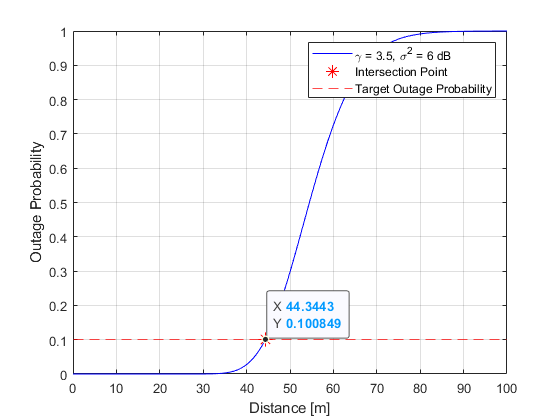
\includegraphics[width=0.8\textwidth]{outage.png}
    \caption{Outage Probability vs Distance}
    \label{fig:outage}
\end{figure}

\subsection*{Part b: Coverage Rate Plot}
The coverage rate represents the probability that the received signal power is above the threshold. It is the complement of the outage probability and is plotted against distance.

\begin{figure}[h]
    \centering
    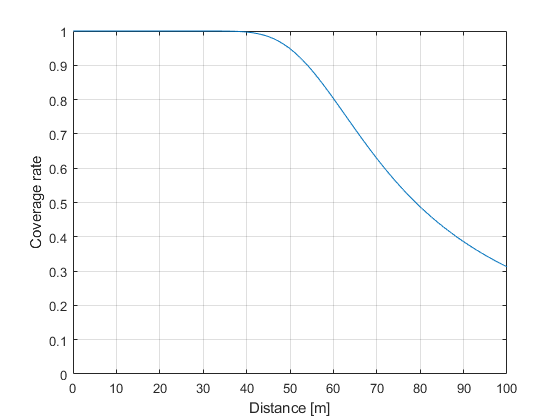
\includegraphics[width=0.8\textwidth]{coverage.png}
    \caption{Coverage Rate vs Distance}
    \label{fig:coverage}
\end{figure}

\subsection*{Part c: Maximum Outage Probability Distance}
To determine the distance at which the maximum outage probability is 0.1, the outage probability is calculated at each distance, and the first instance where it falls below or equal to 0.1 is identified.

\textbf{Result:} The distance at which the maximum outage probability is 0.1 is found to be 44.3443 meters.


\appendix
\section*{Appendix: MATLAB Code}
The following MATLAB code was used for generating the outage probability and coverage rate plots, as well as for calculating the distance at which the maximum outage probability is 0.1.

\begin{verbatim}
clc
clear 
close all
sigma = 6; % Shadowing variance in dB
d_max = 200; % Define the maximum distance
d = 1:d_max; % Distance vector from 1 to d_max meters
P_rx_threshold = -70; % Threshold received power in dBm

% Assuming the same simplified path loss model as before
gamma = 3.5; % path loss exponent
P_tx_dbm = 20; % Transmit power in dBm
L0 = 29.225; % path loss at reference distance

% Calculate the received power at each distance
P_rx = P_tx_dbm - (10*gamma*log10(d) + L0);

% Calculate the outage probability using the Q-function
outage_probability = qfunc((P_rx_threshold - P_rx)/(sigma/sqrt(2)));

% Plotting Outage Probability
figure;
plot(d, 1 - outage_probability);
xlabel('Distance (m)');
ylabel('Outage Probability');
title('Outage Probability vs Distance');
grid on;

% Calculate and Plot Coverage Rate
coverage_rate = outage_probability;

figure;
plot(d, coverage_rate);
xlabel('Distance (m)');
ylabel('Coverage Rate');
title('Coverage Rate vs Distance');
grid on;

% Find the distance where outage probability is 0.1
distance_for_outage = find(outage_probability <= 0.9, 1, 'first');

% Display the result
disp(['Distance for maximum outage probability of 0.1: ', 
      num2str(distance_for_outage), ' meters']);

clc
clear
close all

c = 3e8;
Gt = 9;
Gr = 2;
f = 2.45E9;
d = linspace(0,100,1000);
d0 = 1;
gamma = 3.5;
Pmin = -70;
Pt = 20;
fMhz = f/1e6;
rkm = d;

Pfspl = 20*log10(d0)+20*log10(f)-147.55-Gt-Gr;
Psimplified = Pfspl + 10*gamma*log10(d) - 10*gamma*log10(d0);

Poutage = 1-qfunc((Pmin-(Pt-Psimplified))/sqrt(6));

% Find the distance where the outage probability is 0.1
target_outage = 0.1;
[~, idx] = min(abs(Poutage - target_outage));
intersection_distance = rkm(idx);
intersection_outage = Poutage(idx);

% Plotting
plot(rkm, Poutage, 'b-', 'DisplayName', ['\gamma = ' num2str(gamma), ', \sigma^2 = ' num2str(6) ' dB']);
xlabel('Distance [m]');
ylabel('Outage Probability');
grid on;
hold on;

% Mark the intersection point
plot(intersection_distance, intersection_outage, 'r*', 'MarkerSize', 10, 'DisplayName', 'Intersection Point');

% Draw a line at outage probability of 0.1
yline(target_outage, 'r--', 'DisplayName', 'Target Outage Probability');

legend show;

\end{verbatim}

\end{document}